\documentclass[professionalfonts,aspectratio=169]{beamer}

% ---- Black & white academic styling ----
\usetheme{default}
\usefonttheme{serif} % use roman (Times) font for slide text, not the default sans
\usecolortheme{dove}
\setbeamercolor{structure}{fg=black}
\setbeamercolor{normal text}{fg=black,bg=white}
\setbeamertemplate{navigation symbols}{} % remove nav icons
\setbeamertemplate{footline}[frame number]


% ---- Packages (NO 'caption', NO 'enumitem') ----
\usepackage{amsmath, amssymb, bm, mathtools, mathrsfs, bbm}
\usepackage{mathptmx} % Times New Roman for text and math (pdfLaTeX/Overleaf-safe)
\usepackage{graphicx}
% Images live in latex/imgs (no symlink — Overleaf does not support symlinks).
% Resolve "imgs/chX/..." against the sibling latex/ directory.
\graphicspath{{../latex/}}
\usepackage{booktabs}
\usepackage{microtype}
\usepackage{tikz}
\usetikzlibrary{positioning,fit,backgrounds}
\usepackage{hyperref}
\hypersetup{colorlinks=true, linkcolor=blue}

% =====================================================================
% MAIN QUESTION FOR THE SUPERVISOR (decide first — NOT a slide)
% ---------------------------------------------------------------------
% The reference research project CONTINUED AFTER thesis submission, and
% two of the strongest points (slides 16 and 21) are post-submission
% findings. This forces one decision that shapes the whole talk:
%
%   Should the presentation be restricted to the content of the
%   submitted thesis, or include the continued research — even though
%   that pushes the narrative (and likely the time) beyond the thesis?
%
%   Option A — thesis-only: safest, fully defensible against "is this in
%     your thesis?"; keeps to 20 min. Slides 16/21 use only submitted
%     results.  <-- THIS DECK IS BUILT AS OPTION A (default).
%   Option B — include continued work: stronger story (sharper SOTA
%     framing + a concrete working fix for the main failure mode), shows
%     the research is alive; risks scope/time questions.
%
% Every [POST-SUBMISSION] block is present below but COMMENTED OUT.
% Switch to Option B by uncommenting the marked blocks on slides 16, 21
% and the conclusion.
% =====================================================================

% ---- Title metadata ----
\title{Two Eyes and One Mouth:}
\subtitle{a Training-Free Pipeline with Agentic Image Segmentation and \\ 
Object Video Tracking for Cross-View Object Correspondence}
\author{Marco Lomele}
\institute{Bocconi University --- MSc in Data Science and Business Analytics}
\date{21st July 2026}
\newcommand{\supervisor}{Chiara Plizzari}

\begin{document}

% =====================================================================
% Slide 1 — Title
% =====================================================================
\begin{frame}[plain]
  \begin{center}
    {\LARGE \inserttitle}\\[1.2em]
    {\large \insertsubtitle}\\[1.5em]
    
\includegraphics[width=0.85\textwidth]{imgs/ch1/lang-as-bridge-intro.png}\\[1.2em]
    {\normalsize MSc Thesis\\ \insertauthor \\ Supervised by Prof. \supervisor}
  \end{center}
\end{frame}
\note{(~20s) Good morning, and thank you for being here. My name is Marco Lomele. My thesis is titled "Two Eyes and One Mouth", a training-free pipeline for matching objects across camera views. Let me show you what that means.}

% #####################################################################
\section{Introduction}
% #####################################################################

\begin{frame}{}
    \begin{center}
        $\text{Introduction.}$
    \end{center}
\end{frame}

% =====================================================================
% Slide 2 — The problem: cross-view object correspondence
% =====================================================================
\begin{frame}{Cross-view object correspondence}
  \begin{columns}
    \begin{column}{0.5\textwidth}
      \begin{itemize}
        \item Same object, two synchronized cameras: egocentric and exocentric.
        \item Given the object's mask track in one view, recover it in the other.
        \item Applied in AR, robotics, in general collaboration between agents with vision.
      \end{itemize}
    \end{column}
    \begin{column}{0.5\textwidth}
      
\includegraphics[width=\textwidth]{imgs/ch1/cross-view-intro.png}
    \end{column}
  \end{columns}
\end{frame}
\note{(~55s) So, here is the problem. We have one object, seen by two synchronized cameras. One is egocentric, worn on the head, filming from the wearer's own eyes. The other is exocentric, a camera watching the scene from across the room. I am given the object's mask track in one view, and I have to recover it in the other. Think of the object a person holds in their own hands; I need to find that same object in the camera filming them, and the other way around. Why does this matter? Because any system where two agents must share what they see needs exactly this, from augmented reality to robotics to a robot and a person working together. They all rely on agreeing which object is which.}

% =====================================================================
% Slide 3 — Why it is hard, and where prior methods fall short
% =====================================================================
\begin{frame}{Ego-Exo4D Benchmark}
  \begin{itemize}
    \item Extreme changes in scale, angle, lighting, field of view; no geometric calibration.
    \item Previous methods train modules and rely on abstract vector representations. 
  \end{itemize}
  \begin{center}
    
\includegraphics[width=0.8\textwidth]{imgs/ch1/egoexo-many-examples.png}
  \end{center}
\end{frame}
\note{(~55s) Now, why is this hard? The gap between the two views is extreme. The scale changes, the angle changes, the lighting, the field of view, and we have no geometric calibration tying the cameras together. So classical geometric matching simply breaks. The existing methods take a different route; they train a model to fuse the two views. That works, but it buys accuracy with supervision that does not transfer. Change the cameras, change the dataset, and you retrain from scratch. Worse, their decisions live in opaque weights. When they get an object wrong, you cannot ask them why. These two pains set up my two design goals: no training, and legibility.}

% =====================================================================
% Slide 4 — Our idea: language as a bridge
% =====================================================================
\begin{frame}{Language as a bridge}
  \begin{columns}
    \begin{column}{0.52\textwidth}
      \begin{itemize}
        \item View-independent textual descriptions guide segmentation in the other view.
        \item Pipeline composed of foundation models all used at inference.
        \item Contribution: training-free pipeline testing novel language as bridge paradigm.
      \end{itemize}
    \end{column}
    \begin{column}{0.48\textwidth}
      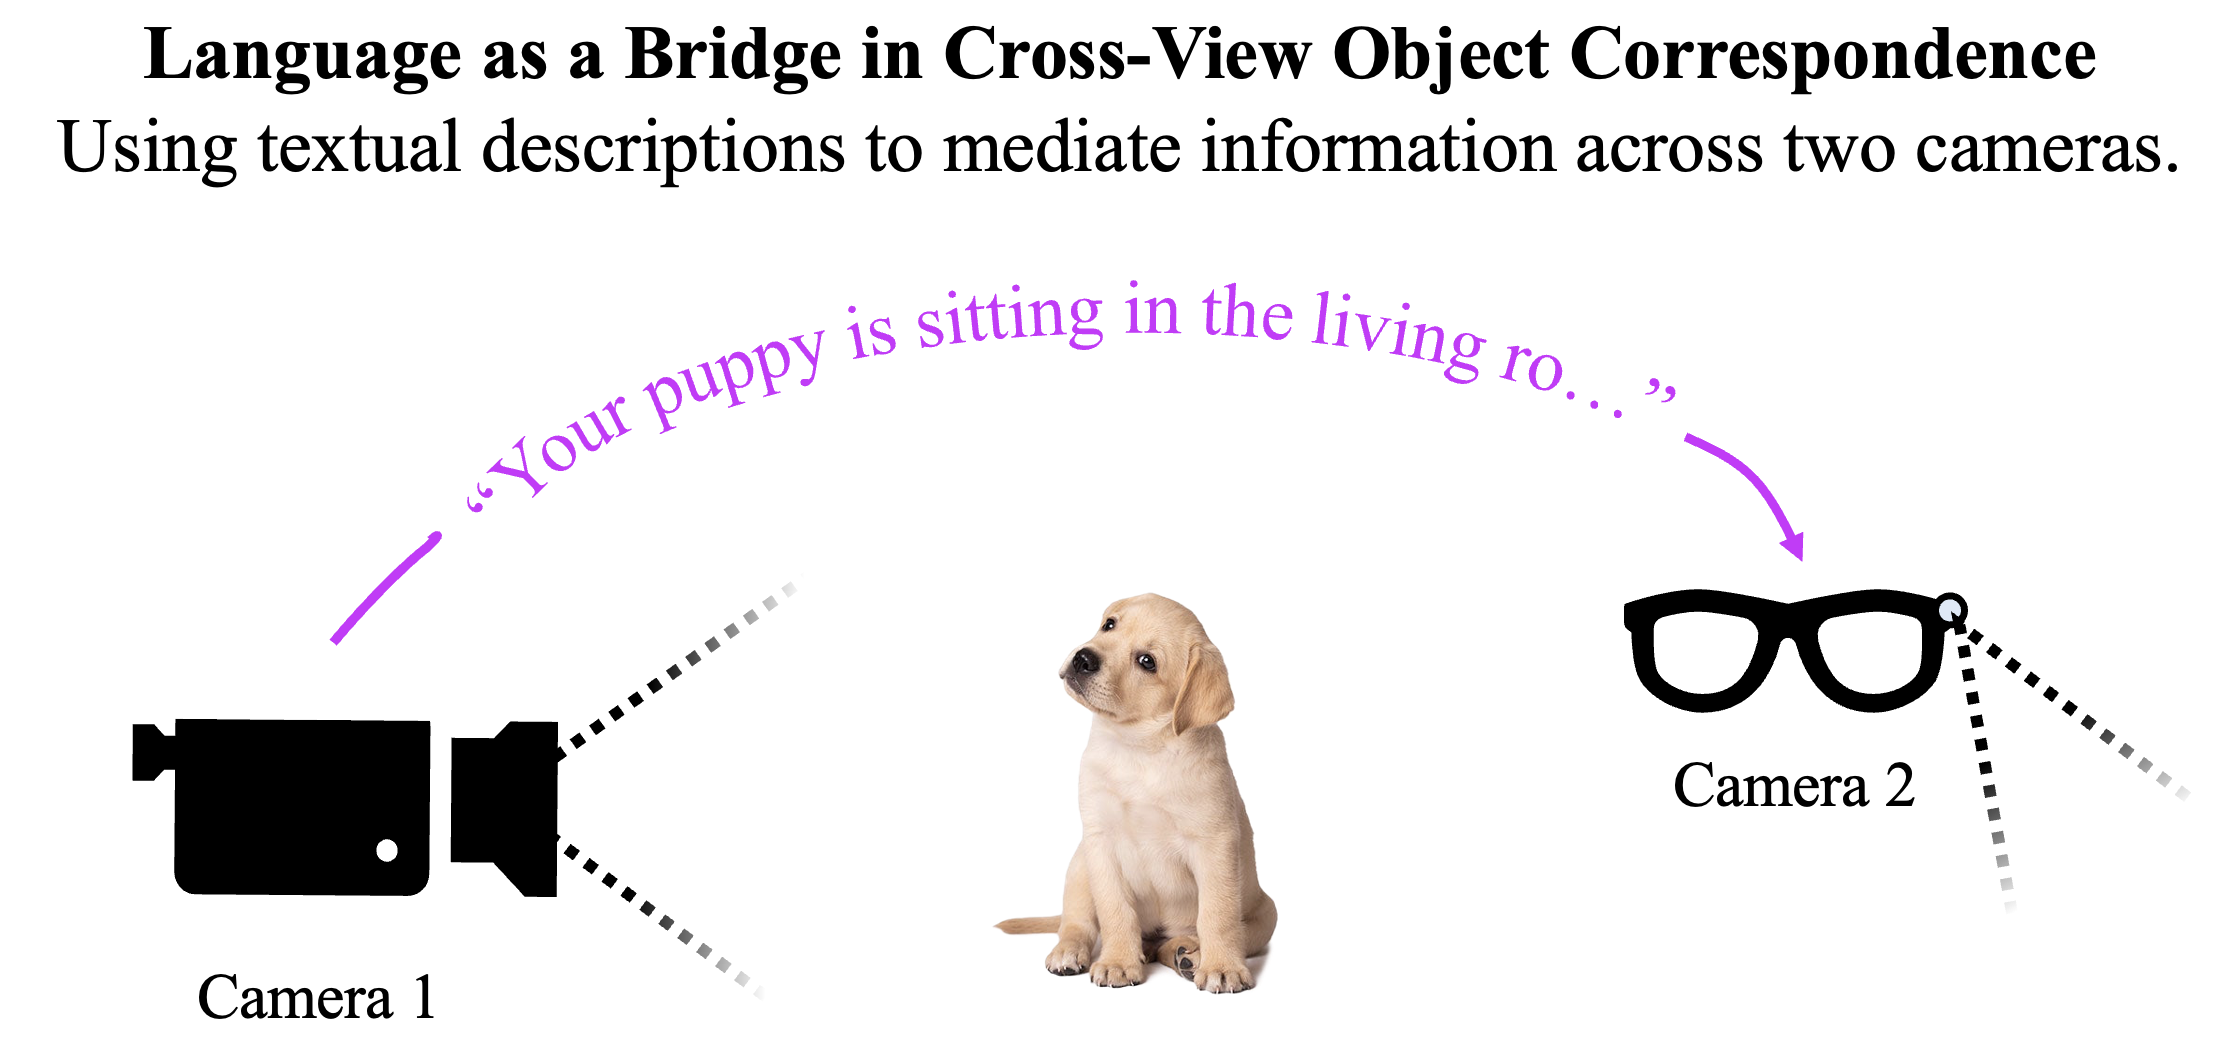
\includegraphics[width=\textwidth]{imgs/ch1/lang-bridge-intro.png}
      
\includegraphics[width=\textwidth]{latex/imgs/ch2/teaser.png}
    \end{column}
  \end{columns}
\end{frame}
\note{(~60s) So here is the idea. What if I describe the object in one view, in plain language, and then find it in the other view through that same description? My hypothesis is that natural language is a semantic channel that survives the viewpoint gap. A change in scale destroys pixels; it does not destroy the words "a red mug". This is the "two eyes and one mouth" in the title, two visual systems mediated by one description. Everything is built from frozen foundation models, composed together, never trained for this task. And the contribution is fourfold. It trains nothing, it bridges through language, every intermediate output is interpretable, and it is agnostic to both the cameras and the dataset.}

% #####################################################################
\section{Theory}
% #####################################################################
\begin{frame}{}
    \begin{center}
        $\text{Theory Review.}$
    \end{center}
\end{frame}

% =====================================================================
% Slide 5 — Visual representation
% =====================================================================
\begin{frame}{Visual representation}
  \begin{columns}
    \begin{column}{0.52\textwidth}
      \begin{itemize}
        \item \textbf{Purpose:} encode an image as fixed-length embeddings; ViT tokenizes patches, self-supervised DINO learns semantic features with no labels.
        \item \textbf{Relevance:} representing images as vectors lets us process them with machine learning.
        \item \textbf{Strengths:} features carry object identity and its relationships with other objects in a scene.
        \item \textbf{Weaknesses:} features grow inconsistent across the extreme ego and exo perspectives, so naive image embeddings cannot be relied on alone.
      \end{itemize}
    \end{column}
    \begin{column}{0.48\textwidth}
      
\includegraphics[width=\textwidth]{imgs/ch2/dinov3-results.png}
    \end{column}
  \end{columns}
\end{frame}
\note{(~50s) Let me walk through the building blocks, four boxes each. What it does, why I use it, what it gives me, and where it breaks. First, visual representation. A Vision Transformer cuts the image into patches and encodes it as fixed-length vectors; DINO learns these features with no labels at all. I need this because once images are vectors, I can compare them with machine learning. And these features are good; they carry object identity, and how an object relates to its surroundings. But here is the weakness that matters most. Across the extreme gap between ego and exo, even the strongest visual features collapse. So I cannot rely on naive image matching alone. That limitation is exactly what pushes me toward language. The whole thesis is a response to it.}

% =====================================================================
% Slide 6 — Segmentation
% =====================================================================
\begin{frame}{Segmentation}
  \begin{columns}
    \begin{column}{0.52\textwidth}
      \begin{itemize}
        \item \textbf{Purpose:} predict a binary object mask.
        \item \textbf{Relevance:} the concrete task we execute on the destination frames, conditioned on information coming from the other view.
        \item \textbf{Strengths:} SAM makes it promptable; SAM 2 adds memory to propagate masks through video; SAM 3 tracks concepts from text prompts. 
        \item \textbf{Weaknesses:} no native cross-view ability.
      \end{itemize}
    \end{column}
    \begin{column}{0.48\textwidth}
      
\includegraphics[width=\textwidth]{latex/imgs/ch2/sam1-examples.png}
    \end{column}
  \end{columns}
\end{frame}
\note{(~50s) Second, segmentation, predicting a binary mask of the object. This is the concrete thing I actually execute on the destination frames. SAM made segmentation promptable, and SAM 2 added memory, so it can propagate a mask through an entire video. Its strength is exactly that temporal tracking, robust through occlusion and fast motion, at constant cost per frame. So I delegate temporal completeness to it. But the weakness mirrors the strength. That same fidelity means if I hand it a wrong seed, it propagates the wrong answer perfectly. Keep this in mind. Later it explains why propagation causes essentially zero percent of my failures, and yet cannot rescue a bad anchor either.}

% =====================================================================
% Slide 7 — Language grounding
% =====================================================================
\begin{frame}{Language grounding}
  \begin{columns}
    \begin{column}{0.54\textwidth}
      \begin{itemize}
        \item \textbf{Purpose:} map a phrase to pixels; CLIP aligns image and text, G-DINO localizes a phrase to a box, SAM 3 turns it into masks.
        \item \textbf{Relevance:} the base of the language bridge, since a description is invariant to viewpoint and carries object identity across the gap where visual features fail.
        \item \textbf{Strengths:} open-vocabulary localization from words; SAM 3 detects, segments and tracks every instance.
        \item \textbf{Weaknesses:} CLIP aligns whole image to whole caption, so long attribute paragraphs dilute the match; SAM 3 is trained on short ($\le$32-token) phrases.
      \end{itemize}
    \end{column}
    \begin{column}{0.46\textwidth}
      
\includegraphics[width=\textwidth]{latex/imgs/ch2/sam3-pcs.png}
    \end{column}
  \end{columns}
\end{frame}
\note{(~55s) Third, language grounding, turning a phrase into pixels. CLIP aligns images and text in one space, Grounding DINO localizes a phrase to a box, and SAM 3 turns that into masks. This is the base of the language bridge, because a description is invariant to viewpoint, so it carries identity across the gap where visual features failed. The strength is localization from an open vocabulary, straight from words. But here is the detail that matters. CLIP aligns the whole image to the whole caption, so a long paragraph of attributes actually dilutes the match, while a short noun phrase concentrates it. And SAM 3 was trained on short phrases, under 32 tokens. So two of my design choices fall directly out of this. Stage 3 compresses the description into a phrase, and the SAM 3 agent, on the next slide, exists to get past that token limit.}

% =====================================================================
% Slide 8 — Foundation models and agents
% =====================================================================
\begin{frame}{Foundation models and agents}
  \begin{columns}
    \begin{column}{0.52\textwidth}
      \begin{itemize}
        \item \textbf{Purpose:} a VLM reasons over image and text; ReAct is a reason $\to$ act $\to$ observe framework for defining agents, namely MLLMs with tools.
        \item \textbf{Relevance:} produces the language bridge and lets the SAM 3 agent segment complex prompts while it self-verifies its masks.
        \item \textbf{Strengths:} instruction following yields consistent descriptions; verification is built in; the reasoning trace keeps every decision legible.
        \item \textbf{Weaknesses:} limited precision under visual prompting, not trained for cross-view correspondence.
      \end{itemize}
    \end{column}
    \begin{column}{0.48\textwidth}
      
\includegraphics[width=\textwidth]{imgs/ch2/react-scheme.png}
      
\includegraphics[width=\textwidth]{latex/imgs/ch2/qwen-training.png}
    \end{column}
  \end{columns}
\end{frame}
\note{(~55s) Fourth, foundation models and agents. A vision-language model reasons jointly over an image and text. ReAct wraps it in a loop, reason, act, observe, so it can call tools and self-correct. I use this in two places: the VLM writes the object description, and the SAM 3 agent segments complex prompts while verifying its own masks. The strengths are real: consistent descriptions, built-in verification, and a reasoning trace that keeps every decision legible. But the weakness foreshadows my dominant failure mode. The model reports what it perceives, not what is annotated. When the target is tiny, it honestly names the larger, salient neighbour it can actually see. That is a perceptual limit, not a hallucination, and we return to it as the single largest source of error.}

\begin{frame}{Segmentation with Complex Prompts}
\begin{center}
    
\includegraphics[width=0.8\textwidth]{latex/imgs/ch2/sam3-agent-examples.png}
\end{center}
\end{frame}
\note{(~30s) Here is what the agent buys me in practice. SAM 3 alone takes a short phrase; on a long, complex description it stumbles. Wrapping it in a reasoning loop lets it break the prompt down, try, check, and retry. So I can segment objects that no single short phrase would have caught.}

% #####################################################################
\section{Method}
% #####################################################################

\begin{frame}{}
    \begin{center}
        $\text{Method.}$
    \end{center}
\end{frame}

% =====================================================================
% Slide 9 — Task formulation and the key insight
% =====================================================================
\begin{frame}{Task formulation}
  \textbf{Input:} video from source camera $\textbf{I}^s$ of $T$ frames and binary mask for each annotated frame:
  \[
    \bigl\{ M_\tau^S \bigr\}_{\tau \in \mathit{T}}, \qquad M_\tau^S \in \{0,1\}^{H \times W}
  \]
  \textbf{Output:} a mask for every frame of destination video $\textbf{I}^D$:
  \[
    \hat{M}_\tau^D \quad \forall\, \tau \in \{1,\ldots,T\}
  \]
  \medskip
  Two problems:
  \begin{itemize}
    \item \textit{Cross-view transfer}: segment the object in one view conditioned on the mask from the other view. 
    \item \textit{Temporal completeness}: predict on every frame.
  \end{itemize}
  \medskip
\textbf{Our pipeline:} language bridge for transfer; SAM 2 for completeness.
\end{frame}

\note{(~50s) Now the method. If you remember one idea from this talk, let it be this one. The input is an object mask track in the source view; the output is a mask for every destination frame. This splits into two orthogonal sub-problems. One is cross-view transfer, getting the object across the viewpoint gap, and that is hard. The other is temporal completeness, covering every frame, and that one is essentially solved by trackers. So my strategy is simple. I spend all my effort on transfer, through language, and I delegate completeness to SAM 2. Every design choice downstream follows from this split.}

% =====================================================================
% Slide 9b — Related works
% =====================================================================
\begin{frame}{Related works}
  \begin{center}
    
\includegraphics[width=0.9\textwidth]{latex/imgs/ch2/related-works.png}
  \end{center}
\end{frame}
\note{}

% =====================================================================
% Slide 10 — Pipeline overview
% =====================================================================
\begin{frame}{Pipeline overview}
  4 stages:
  \begin{enumerate}
      \item Seed Frame Selection
      \item Target Object Description
      \item SAM 3 Agentic Grounding (Anchor Selection + Segmentation) 
      \item Predicted Mask Propagation
  \end{enumerate}
\end{frame}
\note{(~40s) Here is the full pipeline, left to right. Four stages: I select a source frame, describe the object, ground that description into an anchor in the other view, and propagate. The thing I want to stress is legibility. The seed frame, the description, the anchor masks, every intermediate output is something a human can read and inspect. Now let me go through the stages quickly.}

% =====================================================================
% Slide 11 — Stage 1: source frame selection (rapid)
% =====================================================================
\begin{frame}{Stage 1: Source Frame Selection}
  \begin{center}
  
\includegraphics[width=0.8\textwidth]{latex/imgs/ch3/block-1-focus.png}
  \end{center}
  Visibility Scorer computes score $s_\tau$:
  \[
    s_\tau = 0.99\,a_\tau + 0.01\,c_\tau, \qquad
    a_\tau = \frac{A_\tau}{H \cdot W}, \qquad
    c_\tau = 
    1 -
    \frac{\sqrt{\left(c_{y,\tau} - \frac{H}{2}\right)^2 +
    \left(c_{x,\tau} - \frac{W}{2}\right)^2}
    }{\sqrt{\left(\frac{H}{2}\right)^2 +
    \left(\frac{W}{2}\right)^2}},
  \]
  \hspace{4mm} where $a_\tau$ is the normalised mask area and $c_\tau$ is the mask's centrality.
\end{frame}

\note{(~30s) Stage one, source frame selection. I pick the clearest frame by a visibility score, dominated by object area. A bigger object simply gives the VLM more to describe. One good frame is enough, so I take just one. The mechanics I am happy to take in questions.}

% =====================================================================
% Slide 12 — Stage 2: object description (rapid)
% =====================================================================
\begin{frame}{Stage 2: Target Object Description}
  \begin{center}
    
\includegraphics[width=0.9\textwidth]{latex/imgs/ch3/block-2-focus.png}
  \end{center}
\end{frame}
\note{(~30s) Stage two, the description. The VLM writes down only intrinsic attributes, independent of view and of time, so the description holds from any angle, at any moment. It sees the masked frame, which points it at the right object, and the raw frame, which preserves the true appearance. In goes the image, out comes structured JSON.}

% =====================================================================
% Slide 13 — Stage 3: anchor grounding (rapid)
% =====================================================================
\begin{frame}{Stage 3.1: Anchor Selection}
  \begin{center}
    
\includegraphics[width=0.85\textwidth]{latex/imgs/ch3/block-3-1-focus.png}
  \end{center}
\end{frame}
\note{(~40s) Stage three, anchor grounding. Grounding DINO takes the description and re-selects the best anchors by confidence in the destination view; I keep the top three. Then the SAM 3 agent segments them and verifies itself. One line of reasoning to keep. The matching time index is rarely the best destination frame, the correlation is only 0.14, so re-selecting really matters. And notice the bridge stays linguistic here, but the anchor signal is swappable; I could plug in geometry, like RoMa, instead.}

\begin{frame}{Stage 3.2: Agentic Segmentation}
  \begin{center}
    
\includegraphics[width=0.7\textwidth]{latex/imgs/ch3/block-3-2-focus.png}
  \end{center}
\end{frame}
\note{(~30s) Here is the segmentation in detail. It is a loop. The agent proposes a prompt, generates candidate masks, validates them against the description, and selects the best, iterating until it is satisfied. This is how I get a reliable mask out of SAM 3 even on a complex object.}

% =====================================================================
% Slide 14 — Stage 4: propagation (rapid)
% =====================================================================
\begin{frame}{Stage 4: Predicted Mask Propagation}
  \begin{center}
    
\includegraphics[width=0.9\textwidth]{latex/imgs/ch3/block-4-focus.png}
  \end{center}
\end{frame}
\note{(~30s) Stage four, propagation. The SAM 2 memory tracker fills in every remaining frame. It runs in both directions, and each frame is served by its nearest reliable anchor. When the frames nearby fail, memory can reach back to a distant good anchor. The two passes meet, so every single frame has a short path to a solid anchor.}

% #####################################################################
\section{Results \& Analysis}
% #####################################################################

\begin{frame}{}
    \begin{center}
        $\text{Experiments.}$
    \end{center}
\end{frame}

% =====================================================================
% Slide 15 — Setup and qualitative successes
% =====================================================================
\begin{frame}{Experimental notes}
  \begin{itemize}
    \item Frame selections: 1 seed, 3 anchors.
    \item Metrics: IoU, LE, CA.
    \item Inference: NVIDIA H200.
    \item VLM: Qwen 3.5 35B.
  \end{itemize}
\end{frame}
\note{(~55s) Now the results, and this is really the heart of the talk. I evaluate on the Ego-Exo4D Correspondences benchmark, version two, the test split. The primary metric is IoU. Everything runs only at inference, on a single H200 GPU, composing Qwen, Grounding DINO, SAM 3, and SAM 2. And I want to underline this. Not a single component is trained for this task, unlike every competitor on the board. Before the aggregate numbers, look at these, clean successes in both directions, ego-to-exo and exo-to-ego.}

% =====================================================================
% Slide 16 — Results vs. state of the art
% =====================================================================
\begin{frame}{Qualitative results}
\begin{center}

\includegraphics[width=0.85\textwidth]{imgs/ch4/pipeline-qualitative-examples.png}
\end{center}
\end{frame}


\begin{frame}{Quantitative Results}
\begin{center}
    
\includegraphics[width=0.9\textwidth]{latex/imgs/ch4/results-commented.png}
\end{center}
\end{frame}
\note{(~80s) So how does it compare? My pipeline reaches 37.7 IoU ego-to-exo and 40.6 exo-to-ego, and it trains nothing. That already beats ObjectRelator, and mine is the only method that is at once free of training, agnostic to the camera, and agnostic to the dataset. The strongest published result is LM-EEC, at roughly 55 and 66, and I present it plainly as the strongest published number. I sit a few points back on raw IoU, but I pay none of the supervision cost, and I generalize where they cannot. Now, let me show you that this raw gap hides something much more interesting. [Option A framing: strongest-published, no upper-bound argument.]}  
% === POST-SUBMISSION (Option B) — uncomment if supervisor approves ===
% Replace the bullets above with:
%   \item Ours: 37.7 (Ego2Exo) / 40.6 (Exo2Ego) IoU --- training-free.
%   \item Realistic comparator $\to$ V$^2$-SAM: 46.3 / 49.6 (no backbone retraining on the benchmark).
%   \item In-distribution ceiling $\to$ LM-EEC: 54.98 / 65.77 (full SAM 2 fine-tuned on the benchmark).
%   \item We beat ObjectRelator (35.3 / 40.3); only method training-free + camera- + dataset-agnostic.
% And the note:
%   (~80s) Frame the two comparators differently -- this is the analytical point, not the raw
%   gap. LM-EEC is an in-distribution upper bound: it fine-tunes the full SAM 2 backbone on the
%   benchmark, so its number reports what a retrained model achieves on data it has seen, not what
%   a fair like-for-like method achieves. The honest comparator is V^2-SAM, which does not retrain
%   a backbone; against that frontier our training-free pipeline sits a few points back while
%   paying none of the supervision cost.
% === end POST-SUBMISSION ===

% =====================================================================
% Slide 17 — Ablation: what each stage contributes
% =====================================================================
\begin{frame}{Contribution of each stage}
  \begin{itemize}
    \item Baseline: query the VLM independently on every source frame and run one-shot SAM 3 per destination frame.
    \item Baseline Oracle: baseline substituting VLM descriptions with object labels from metadata. 
  \end{itemize}
  \begin{center}
    \small
    \setlength{\tabcolsep}{10pt}
    \renewcommand{\arraystretch}{1.1}
    \begin{tabular}{lrr}
      \toprule
      Stage added & IoU$\uparrow$ & $t$/frame\,(s)$\downarrow$ \\
      \midrule
      Baseline            & 10.6 & 1.32 \\
      Baseline Oracle     & 17.0 & 0.12 \\
      \midrule
      (A) Best Single Frame & 16.8 & 0.13 \\
      (B) SAM3 Agent Loop   & 35.5 & 21.30 \\
      (C) Propagation       & 37.7 & 0.82 \\
      (D) G-DINO            & \textbf{38.1} & 0.90 \\
      \midrule
      \% change vs. Baseline
        & \textcolor[rgb]{0,0.55,0}{$+259.8\%$}
        & \textcolor[rgb]{0,0.55,0}{$-31.8\%$} \\
      \bottomrule
    \end{tabular}
  \end{center}
\end{frame}
\note{(~70s) This ablation validates the design split. A naive baseline sits at 10.6 IoU; the full pipeline lifts that by 260 percent. Two rows matter most. My frame selection, with no privileged information, essentially matches an oracle, 16.8 against 17.0. And propagation matches running the SAM 3 agent on every single frame, 37.7 against 35.5, but at twenty-five times the speed, under a second per frame instead of twenty-one. Running the agent on every frame would take 59 hours; propagation recovers the same accuracy for almost nothing. The numbers say the split was the right call.}

% =====================================================================
% Slide 18 — The gap is bimodal
% =====================================================================
\begin{frame}{The gap to SOTA}
  \begin{columns}
    \begin{column}{0.5\textwidth}
      \begin{itemize}
        \item $\sim$32\% (Ego2Exo) / 31\% (Exo2Ego) ``dead mass'': near-zero IoU.
        \item Surviving cases (working mode): 56.9 / 61.7 IoU.
        \item Remove the dead mass $\to$ mean IoU rises $\sim$18, level with LM-EEC.
      \end{itemize}
    \end{column}
    \begin{column}{0.5\textwidth}
      
\includegraphics[width=0.9\textwidth]{imgs/ch4/pipeline-lmeec.png}
    \end{column}
  \end{columns}
\end{frame}
\note{(~75s) Now look closer at the gap to the state of the art, because it is not what it seems. The errors are bimodal. About a third of cases, 32 percent ego-to-exo and 31 percent the other way, are what I call "dead mass", near-zero IoU, total failures. But the cases that survive, the working mode, score 56.9 and 61.7. That is already level with the state of the art. So the deficit is not uniform sloppiness; it is half clean failure and half ordinary error. If I could simply remove the dead mass, my average jumps by about 18 points, right up to LM-EEC. So the whole question becomes one thing. What causes the dead mass?}

% =====================================================================
% Slide 19 — Where the loss is born
% =====================================================================
\begin{frame}{Dead mass}
  \begin{itemize}
    \item Bottle Neck: stage 2 naming, responsible for 59\% (Ego2Exo) / 81\% (Exo2Ego) of dead mass.
  \end{itemize}
  \begin{center}
    
\includegraphics[width=0.8\textwidth]{imgs/ch4/grounding-examples.png}
  \end{center}
\end{frame}
\note{(~70s) To answer that, I charge each failure to the first stage where it goes wrong. The result is stark. Stage two, the naming itself, accounts for 59 percent of dead mass ego-to-exo and 81 percent the other way. Stages two and three together, 74 and 92 percent. And propagation? Zero percent, by construction. So the loss is born in cross-view transfer, not in tracking. An anchor placed on the wrong object propagates faithfully to a wrong answer. The failure is decided early, at description and grounding, exactly the hard sub-problem I flagged at the start.}

% =====================================================================
% Slide 20 — Why the VLM mislabels: perception, not vocabulary
% =====================================================================
\begin{frame}{Why the VLM mislabels: perception, not vocabulary}
  \begin{itemize}
    \item On dead cases the source mask is 3--6$\times$ smaller; the model names a real, larger neighbour.
    \item It never hallucinates an absent object; the failure is perceptual, not lexical.
  \end{itemize}
  \begin{center}
    
\includegraphics[width=0.8\textwidth]{imgs/ch4/vlm-description-failure.png}
  \end{center}
\end{frame}
\note{(~80s) So why does the VLM mislabel? This is the analytical core. I looked at the dead cases, and the pattern is consistent. The source object's mask is three to six times smaller than usual, and the model names a real, larger neighbour instead. Crucially, it never invents an object that is not there. It does not hallucinate. With too few pixels, it honestly describes the salient surface, or the tool the target is resting on. And that diagnosis matters, because it rules out the obvious fix. The problem is not a poor vocabulary or a weak prompt. The problem is perception; the model simply cannot see a small enough object well enough to name it.}

% =====================================================================
% Slide 21 — Testing the diagnosis: disciplined negatives
% =====================================================================
\begin{frame}{Testing the diagnosis: disciplined negatives}
  \begin{itemize}
    \item Scene-vocabulary conditioning, destination cropping, frame brightening; all tried, all net-negative.
    \item Cropping helps failing frames but corrupts the many already-correct ones; brightening confirms pixels are not the constraint.
    \item Negatives point the same way: the fix must use the VLM better, not pre-process the image.
  \end{itemize}
  \begin{center}
    \small
    \setlength{\tabcolsep}{9pt}
    \renewcommand{\arraystretch}{1.15}
    \begin{tabular}{lccc}
      \toprule
      Intervention & Off & On & $\Delta$ \\
      \midrule
      Scene-vocabulary conditioning & 37.8 & 38.9 & \textcolor[rgb]{0,0.55,0}{$+1.1$} \\
      Destination crop hint          & 37.8 & 33.4 & \textcolor[rgb]{0.7,0,0}{$-4.4$} \\
      Frame brightening              & 37.8 & 34.1 & \textcolor[rgb]{0.7,0,0}{$-3.7$} \\
      \bottomrule
    \end{tabular}

    \vspace{0.4em}
    {\footnotesize \textit{Ego2Exo} IoU, 25\% validation, anchors ranked by confidence.}
  \end{center}
\end{frame}
\note{(~80s) To test that diagnosis, I ran a set of disciplined interventions, and I want to frame these as method, not as a list of misses. I tried conditioning on the scene vocabulary, cropping the destination, and brightening the frame. Every one of them hurt overall. Cropping is telling; it helps the failing frames, but it corrupts the many that were already correct. Brightening confirms that raw pixels are not the constraint. So the negatives are informative precisely because they kill the cheap fixes, vocabulary, cropping, lighting, and isolate the real constraint, which is how the VLM perceives small objects. That is where the answer has to come from. I leave the two concrete fixes that follow from this for future work. [Option A: end on the diagnosis.]}
% === POST-SUBMISSION (Option B) — uncomment if supervisor approves ===
% Add this bullet to the itemize above:
%   \item Two working directions: (i) pass the mask signal into the VLM so it describes the
%         target, not its neighbour; (ii) add a judge layer after SAM 3 to filter candidate
%         masks against the description.
% And extend the note:
%   That diagnosis directly motivated the continued work: feeding the mask signal to the VLM
%   addresses the perceptual mislabel at its source, and a judge stage after SAM 3 catches the
%   confident mis-groundings that have no internal confidence signal.
% === end POST-SUBMISSION ===

% #####################################################################
\section{Conclusion}
% #####################################################################

% =====================================================================
% Slide 22 — Conclusions and future work
% =====================================================================
\begin{frame}{Conclusions and future work}
  \begin{itemize}
    \item Language is a viable cross-view bridge, and, crucially, a legible one.
    \item Legibility turned the gap to SOTA into a diagnosis, not a verdict.
    \item Near-term: description optimization (mask signal to the VLM), stronger grounding, a judge/verification gate.
    \item Paradigm: legibility vs. performance trade-off; composing foundation models rather than training them.
  \end{itemize}
\end{frame}
\note{(~60s) Let me close. I have shown that language is a viable bridge across the viewpoint gap, and, crucially, a legible one. That legibility is what let me turn the gap to the state of the art into a diagnosis rather than a verdict; I can say not just that I lose, but exactly where, and why. In the near term, the path is clear. Optimize the description by passing the mask signal into the VLM, strengthen the grounding, and add a judge to verify masks against the description. But the larger claim is this. As foundation models absorb more and more general understanding, the most capable systems may be ones we compose rather than train, with language as the medium a human can read, the one thing that keeps people in the loop. Thank you.}
% === POST-SUBMISSION (Option B) — uncomment if supervisor approves ===
% Under Option B the two directions were already shown working on slide 21, so here drop the
% "near-term" bullet and instead point forward to the open paradigm questions only.
% === end POST-SUBMISSION ===

\end{document}
